\documentclass[]{article}
\usepackage{lmodern}
\usepackage{amssymb,amsmath}
\usepackage{ifxetex,ifluatex}
\usepackage{fixltx2e} % provides \textsubscript
\ifnum 0\ifxetex 1\fi\ifluatex 1\fi=0 % if pdftex
  \usepackage[T1]{fontenc}
  \usepackage[utf8]{inputenc}
\else % if luatex or xelatex
  \ifxetex
    \usepackage{mathspec}
  \else
    \usepackage{fontspec}
  \fi
  \defaultfontfeatures{Ligatures=TeX,Scale=MatchLowercase}
\fi
% use upquote if available, for straight quotes in verbatim environments
\IfFileExists{upquote.sty}{\usepackage{upquote}}{}
% use microtype if available
\IfFileExists{microtype.sty}{%
\usepackage{microtype}
\UseMicrotypeSet[protrusion]{basicmath} % disable protrusion for tt fonts
}{}
\usepackage[margin=1in]{geometry}
\usepackage{hyperref}
\hypersetup{unicode=true,
            pdftitle={02 Data Structures},
            pdfborder={0 0 0},
            breaklinks=true}
\urlstyle{same}  % don't use monospace font for urls
\usepackage{color}
\usepackage{fancyvrb}
\newcommand{\VerbBar}{|}
\newcommand{\VERB}{\Verb[commandchars=\\\{\}]}
\DefineVerbatimEnvironment{Highlighting}{Verbatim}{commandchars=\\\{\}}
% Add ',fontsize=\small' for more characters per line
\newenvironment{Shaded}{}{}
\newcommand{\AlertTok}[1]{\textcolor[rgb]{1.00,0.00,0.00}{\textbf{#1}}}
\newcommand{\AnnotationTok}[1]{\textcolor[rgb]{0.38,0.63,0.69}{\textbf{\textit{#1}}}}
\newcommand{\AttributeTok}[1]{\textcolor[rgb]{0.49,0.56,0.16}{#1}}
\newcommand{\BaseNTok}[1]{\textcolor[rgb]{0.25,0.63,0.44}{#1}}
\newcommand{\BuiltInTok}[1]{#1}
\newcommand{\CharTok}[1]{\textcolor[rgb]{0.25,0.44,0.63}{#1}}
\newcommand{\CommentTok}[1]{\textcolor[rgb]{0.38,0.63,0.69}{\textit{#1}}}
\newcommand{\CommentVarTok}[1]{\textcolor[rgb]{0.38,0.63,0.69}{\textbf{\textit{#1}}}}
\newcommand{\ConstantTok}[1]{\textcolor[rgb]{0.53,0.00,0.00}{#1}}
\newcommand{\ControlFlowTok}[1]{\textcolor[rgb]{0.00,0.44,0.13}{\textbf{#1}}}
\newcommand{\DataTypeTok}[1]{\textcolor[rgb]{0.56,0.13,0.00}{#1}}
\newcommand{\DecValTok}[1]{\textcolor[rgb]{0.25,0.63,0.44}{#1}}
\newcommand{\DocumentationTok}[1]{\textcolor[rgb]{0.73,0.13,0.13}{\textit{#1}}}
\newcommand{\ErrorTok}[1]{\textcolor[rgb]{1.00,0.00,0.00}{\textbf{#1}}}
\newcommand{\ExtensionTok}[1]{#1}
\newcommand{\FloatTok}[1]{\textcolor[rgb]{0.25,0.63,0.44}{#1}}
\newcommand{\FunctionTok}[1]{\textcolor[rgb]{0.02,0.16,0.49}{#1}}
\newcommand{\ImportTok}[1]{#1}
\newcommand{\InformationTok}[1]{\textcolor[rgb]{0.38,0.63,0.69}{\textbf{\textit{#1}}}}
\newcommand{\KeywordTok}[1]{\textcolor[rgb]{0.00,0.44,0.13}{\textbf{#1}}}
\newcommand{\NormalTok}[1]{#1}
\newcommand{\OperatorTok}[1]{\textcolor[rgb]{0.40,0.40,0.40}{#1}}
\newcommand{\OtherTok}[1]{\textcolor[rgb]{0.00,0.44,0.13}{#1}}
\newcommand{\PreprocessorTok}[1]{\textcolor[rgb]{0.74,0.48,0.00}{#1}}
\newcommand{\RegionMarkerTok}[1]{#1}
\newcommand{\SpecialCharTok}[1]{\textcolor[rgb]{0.25,0.44,0.63}{#1}}
\newcommand{\SpecialStringTok}[1]{\textcolor[rgb]{0.73,0.40,0.53}{#1}}
\newcommand{\StringTok}[1]{\textcolor[rgb]{0.25,0.44,0.63}{#1}}
\newcommand{\VariableTok}[1]{\textcolor[rgb]{0.10,0.09,0.49}{#1}}
\newcommand{\VerbatimStringTok}[1]{\textcolor[rgb]{0.25,0.44,0.63}{#1}}
\newcommand{\WarningTok}[1]{\textcolor[rgb]{0.38,0.63,0.69}{\textbf{\textit{#1}}}}
\usepackage{graphicx,grffile}
\makeatletter
\def\maxwidth{\ifdim\Gin@nat@width>\linewidth\linewidth\else\Gin@nat@width\fi}
\def\maxheight{\ifdim\Gin@nat@height>\textheight\textheight\else\Gin@nat@height\fi}
\makeatother
% Scale images if necessary, so that they will not overflow the page
% margins by default, and it is still possible to overwrite the defaults
% using explicit options in \includegraphics[width, height, ...]{}
\setkeys{Gin}{width=\maxwidth,height=\maxheight,keepaspectratio}
\IfFileExists{parskip.sty}{%
\usepackage{parskip}
}{% else
\setlength{\parindent}{0pt}
\setlength{\parskip}{6pt plus 2pt minus 1pt}
}
\setlength{\emergencystretch}{3em}  % prevent overfull lines
\providecommand{\tightlist}{%
  \setlength{\itemsep}{0pt}\setlength{\parskip}{0pt}}
\setcounter{secnumdepth}{0}
% Redefines (sub)paragraphs to behave more like sections
\ifx\paragraph\undefined\else
\let\oldparagraph\paragraph
\renewcommand{\paragraph}[1]{\oldparagraph{#1}\mbox{}}
\fi
\ifx\subparagraph\undefined\else
\let\oldsubparagraph\subparagraph
\renewcommand{\subparagraph}[1]{\oldsubparagraph{#1}\mbox{}}
\fi

%%% Use protect on footnotes to avoid problems with footnotes in titles
\let\rmarkdownfootnote\footnote%
\def\footnote{\protect\rmarkdownfootnote}

%%% Change title format to be more compact
\usepackage{titling}

% Create subtitle command for use in maketitle
\providecommand{\subtitle}[1]{
  \posttitle{
    \begin{center}\large#1\end{center}
    }
}

\setlength{\droptitle}{-2em}

  \title{02 Data Structures}
    \pretitle{\vspace{\droptitle}\centering\huge}
  \posttitle{\par}
    \author{}
    \preauthor{}\postauthor{}
    \date{}
    \predate{}\postdate{}
  
\usepackage{\string~/Dropbox/profiles/Templates/LaTeX/ScreenStyle}
\usepackage{listings}

\begin{document}
\maketitle

{
\setcounter{tocdepth}{2}
\tableofcontents
}
\hypertarget{practical-02}{%
\section{Practical 02}\label{practical-02}}

\hypertarget{preamble}{%
\subsection{Preamble}\label{preamble}}

\begin{Shaded}
\begin{Highlighting}[]
\CommentTok{## (01) Clean up the Iris Data}

\CommentTok{# Preamble}
\CommentTok{## Install Pacman}
\NormalTok{load.pac <-}\StringTok{ }\ControlFlowTok{function}\NormalTok{() \{}
  
  \ControlFlowTok{if}\NormalTok{(}\KeywordTok{require}\NormalTok{(}\StringTok{"pacman"}\NormalTok{))\{}
    \KeywordTok{library}\NormalTok{(pacman)}
\NormalTok{  \}}\ControlFlowTok{else}\NormalTok{\{}
    \KeywordTok{install.packages}\NormalTok{(}\StringTok{"pacman"}\NormalTok{)}
    \KeywordTok{library}\NormalTok{(pacman)}
\NormalTok{  \}}
  
\NormalTok{  pacman}\OperatorTok{::}\KeywordTok{p_load}\NormalTok{(xts, sp, gstat, ggplot2, rmarkdown, reshape2, ggmap,}
\NormalTok{                 parallel, dplyr, plotly, tidyverse, reticulate, UsingR, Rmpfr,}
\NormalTok{                 swirl, corrplot, gridExtra, mise, latex2exp)}
  
\NormalTok{\}}

\KeywordTok{load.pac}\NormalTok{()}
\end{Highlighting}
\end{Shaded}

\begin{verbatim}
## Loading required package: pacman
\end{verbatim}

\begin{Shaded}
\begin{Highlighting}[]
\KeywordTok{mise}\NormalTok{()}
\end{Highlighting}
\end{Shaded}

\newpage{}

\begin{Shaded}
\begin{Highlighting}[]
\KeywordTok{set.seed}\NormalTok{(}\DecValTok{9823}\NormalTok{)}
\end{Highlighting}
\end{Shaded}

\begin{Shaded}
\begin{Highlighting}[]
\NormalTok{knitr}\OperatorTok{::}\NormalTok{opts_chunk}\OperatorTok{$}\KeywordTok{set}\NormalTok{(}
  \DataTypeTok{fig.path =} \StringTok{"./figure/"}
\NormalTok{)}
\end{Highlighting}
\end{Shaded}

\hypertarget{create-gaussian-values}{%
\subsection{(1) Create Gaussian Values}\label{create-gaussian-values}}

\begin{Shaded}
\begin{Highlighting}[]
\NormalTok{std_normal <-}\StringTok{ }\KeywordTok{rnorm}\NormalTok{(}\DataTypeTok{n =} \DecValTok{20}\NormalTok{, }\DataTypeTok{mean =} \DecValTok{0}\NormalTok{, }\DataTypeTok{sd =} \DecValTok{1}\NormalTok{)}
\KeywordTok{cat}\NormalTok{(std_normal)}
\end{Highlighting}
\end{Shaded}

\begin{verbatim}
## 0.8890603 -0.3824008 -0.1658778 1.52031 -1.382377 1.10355 -0.2035836 -1.77049 -0.7843132 -0.9573273 -0.3120387 1.4742 0.07174706 0.1801898 0.1126159 0.8977332 -0.2474811 1.026038 -1.977872 0.1270891
\end{verbatim}

\hypertarget{manipulate-the-values}{%
\subsection{(2) Manipulate the Values}\label{manipulate-the-values}}

\hypertarget{print-the-number-of-positive-values}{%
\subsubsection{Print the number of Positive
Values}\label{print-the-number-of-positive-values}}

\begin{Shaded}
\begin{Highlighting}[]
\CommentTok{## Using Base Functions}
\NormalTok{n_geq0 <-}\StringTok{ }\NormalTok{std_normal[std_normal}\OperatorTok{>}\DecValTok{0}\NormalTok{]  }\OperatorTok\StringTok{ }\KeywordTok{length}\NormalTok{()}

\NormalTok{n_geq0 <-}\StringTok{ }\NormalTok{std_normal[}\KeywordTok{sign}\NormalTok{(std_normal) }\OperatorTok{==}\StringTok{ }\DecValTok{1}\NormalTok{] }\OperatorTok\StringTok{ }\KeywordTok{length}\NormalTok{()}
\NormalTok{n_neg <-}\StringTok{ }\KeywordTok{length}\NormalTok{(std_normal)}\OperatorTok{-}\NormalTok{n_geq0}

\CommentTok{## Using Dplyr}
\CommentTok{# std_normal %>% dplyr::filter()}


 \KeywordTok{print}\NormalTok{(}\StringTok{"| Positive Values | Negative Values | "}\NormalTok{)}
\end{Highlighting}
\end{Shaded}

\begin{verbatim}
## [1] "| Positive Values | Negative Values | "
\end{verbatim}

\begin{Shaded}
\begin{Highlighting}[]
\KeywordTok{print}\NormalTok{(}\StringTok{"| --------------- | --------------- | "}\NormalTok{)}
\end{Highlighting}
\end{Shaded}

\begin{verbatim}
## [1] "| --------------- | --------------- | "
\end{verbatim}

\begin{Shaded}
\begin{Highlighting}[]
\KeywordTok{paste0}\NormalTok{(}\StringTok{"|     "}\NormalTok{, n_geq0, }\StringTok{"           |     "}\NormalTok{, n_neg, }\StringTok{"           | "}\NormalTok{) }\OperatorTok\StringTok{ }\KeywordTok{print}\NormalTok{()}
\end{Highlighting}
\end{Shaded}

\begin{verbatim}
## [1] "|     10           |     10           | "
\end{verbatim}

\hypertarget{make-all-values-positive}{%
\subsubsection{Make all Values
Positive}\label{make-all-values-positive}}

So the easiest way to do this would be to just use \texttt{abs()} or
\texttt{sqrt(x\^{}2)}, a more programatic way would be to use an if
statement:

\begin{Shaded}
\begin{Highlighting}[]
\NormalTok{std_normal[std_normal}\OperatorTok{<}\DecValTok{0}\NormalTok{]<-}\StringTok{ }\NormalTok{std_normal[std_normal}\OperatorTok{<}\DecValTok{0}\NormalTok{]}\OperatorTok{*-}\DecValTok{1}
\NormalTok{std_normal}
\end{Highlighting}
\end{Shaded}

\begin{verbatim}
##  [1] 0.88906032 0.38240081 0.16587781 1.52030961 1.38237738 1.10355041
##  [7] 0.20358362 1.77049048 0.78431321 0.95732729 0.31203867 1.47419964
## [13] 0.07174706 0.18018983 0.11261591 0.89773317 0.24748110 1.02603848
## [19] 1.97787202 0.12708910
\end{verbatim}

\hypertarget{create-bins}{%
\subsection{(3) Create Bins}\label{create-bins}}

\hypertarget{equal-size-histogram-bins}{%
\subsubsection{Equal Size Histogram
bins}\label{equal-size-histogram-bins}}

Creating 3 bins that are equally sized, from the minimum observation, to
the maximum observation could be acheived thusly:

\begin{Shaded}
\begin{Highlighting}[]
\NormalTok{minval <-}\StringTok{ }\KeywordTok{min}\NormalTok{(std_normal)}
\NormalTok{maxval <-}\StringTok{ }\KeywordTok{max}\NormalTok{(std_normal)}
\NormalTok{delta <-}\StringTok{ }\NormalTok{(maxval}\OperatorTok{-}\NormalTok{minval) }\OperatorTok{/}\StringTok{ }\DecValTok{3}
\NormalTok{break_points <-}\StringTok{ }\KeywordTok{c}\NormalTok{(minval, delta, }\DecValTok{2}\OperatorTok{*}\NormalTok{delta, maxval)}

\CommentTok{#bin_count <- cut(std_normal, breaks = break_points) %>% table()}
\NormalTok{bin_index  <-}\StringTok{ }\KeywordTok{factor}\NormalTok{(}\KeywordTok{cut}\NormalTok{(std_normal, }\DataTypeTok{breaks =}\NormalTok{ break_points))}
\NormalTok{bin_count   <-}\StringTok{ }\KeywordTok{table}\NormalTok{(bin_index) }

\KeywordTok{paste}\NormalTok{(}\StringTok{"The distribution of values across the bins are:"}\NormalTok{) }\OperatorTok\StringTok{ }\KeywordTok{print}\NormalTok{()}
\end{Highlighting}
\end{Shaded}

\begin{verbatim}
## [1] "The distribution of values across the bins are:"
\end{verbatim}

\begin{Shaded}
\begin{Highlighting}[]
\KeywordTok{print}\NormalTok{(bin_count)}
\end{Highlighting}
\end{Shaded}

\begin{verbatim}
## bin_index
## (0.0717,0.635]   (0.635,1.27]    (1.27,1.98] 
##              8              6              5
\end{verbatim}

\hypertarget{plot-the-binned-values}{%
\paragraph{Plot the Binned Values}\label{plot-the-binned-values}}

The bins can be used to pass breaks to a histogram or they can be used
to specify counts for a barplot:

\begin{Shaded}
\begin{Highlighting}[]
\CommentTok{# layout(matrix(1:2, nrow = 2))}

\KeywordTok{hist}\NormalTok{(std_normal, }\DataTypeTok{breaks =}\NormalTok{ break_points, }\DataTypeTok{freq =} \OtherTok{TRUE}\NormalTok{, }\DataTypeTok{main =} \StringTok{"Histogram of Values"}\NormalTok{, }\DataTypeTok{xlab =} \StringTok{"Simulated Normal Value"}\NormalTok{, }\DataTypeTok{col =} \KeywordTok{c}\NormalTok{(}\StringTok{"lightblue"}\NormalTok{, }\StringTok{"pink"}\NormalTok{, }\StringTok{"lightgreen"}\NormalTok{))}
\end{Highlighting}
\end{Shaded}

\begin{verbatim}
## Warning in plot.histogram(r, freq = freq1, col = col, border = border, angle =
## angle, : the AREAS in the plot are wrong -- rather use 'freq = FALSE'
\end{verbatim}

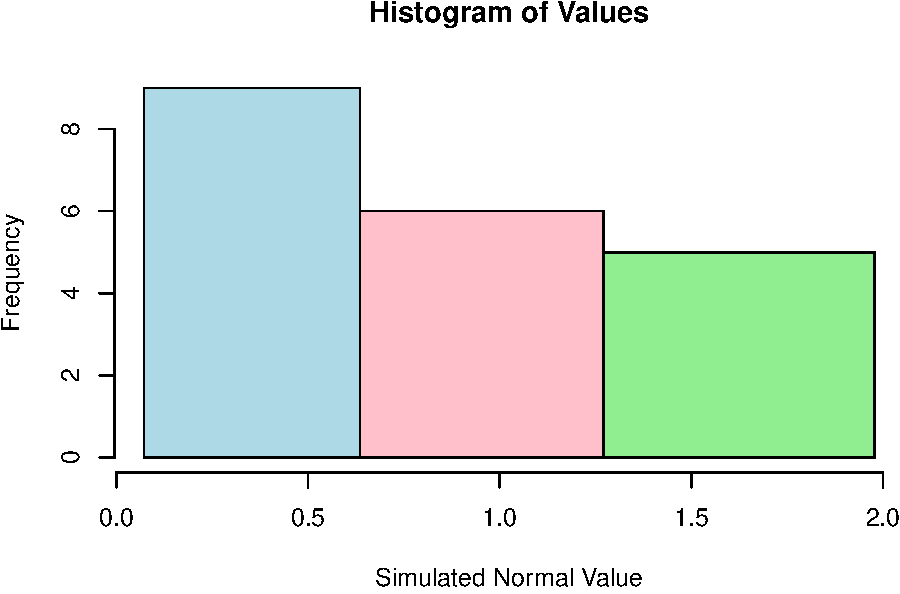
\includegraphics{./figure/unnamed-chunk-7-1.pdf}

\begin{Shaded}
\begin{Highlighting}[]
\KeywordTok{barplot}\NormalTok{(bin_count, }\DataTypeTok{col =} \KeywordTok{c}\NormalTok{(}\StringTok{"lightblue"}\NormalTok{, }\StringTok{"pink"}\NormalTok{, }\StringTok{"lightgreen"}\NormalTok{), }\DataTypeTok{main =} \StringTok{"Bar Plot of Binned Values"}\NormalTok{)}
\end{Highlighting}
\end{Shaded}

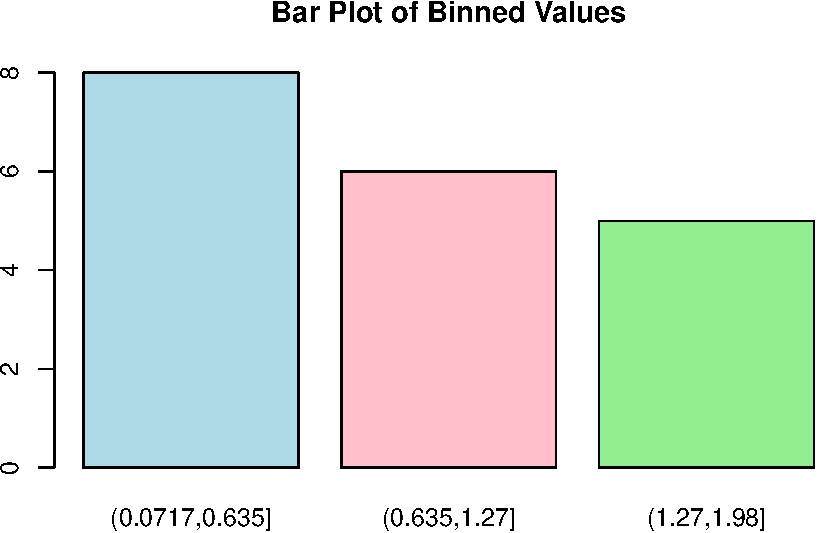
\includegraphics{./figure/unnamed-chunk-7-2.pdf}

\begin{Shaded}
\begin{Highlighting}[]
\KeywordTok{ggplot}\NormalTok{(}\DataTypeTok{data =} \KeywordTok{melt}\NormalTok{(bin_count), }\KeywordTok{aes}\NormalTok{(}\DataTypeTok{x =}\NormalTok{ bin_index, }\DataTypeTok{y =}\NormalTok{ value, }\DataTypeTok{fill =}\NormalTok{ bin_index, }\DataTypeTok{col =} \OperatorTok{-}\NormalTok{value)) }\OperatorTok{+}
\StringTok{  }\KeywordTok{geom_col}\NormalTok{() }\OperatorTok{+}
\StringTok{  }\KeywordTok{guides}\NormalTok{(}\DataTypeTok{col =} \OtherTok{FALSE}\NormalTok{, }\DataTypeTok{fill =} \KeywordTok{guide_legend}\NormalTok{(}\StringTok{"Inter-tierce }\CharTok{\textbackslash{}n}\StringTok{ Range"}\NormalTok{)) }\OperatorTok{+}
\StringTok{  }\KeywordTok{theme_bw}\NormalTok{() }\OperatorTok{+}
\StringTok{  }\KeywordTok{labs}\NormalTok{(}\DataTypeTok{x =} \StringTok{"Interval of bin Values"}\NormalTok{, }\DataTypeTok{title =} \StringTok{"Binned Values"}\NormalTok{, }\DataTypeTok{y =} \StringTok{"Frequency of Value"}\NormalTok{, }
       \DataTypeTok{subtitle =} \StringTok{"Absolute value of normally distributed sample `rnorm`"}\NormalTok{) }\OperatorTok{+}
\StringTok{  }\KeywordTok{scale_fill_brewer}\NormalTok{(}\DataTypeTok{palette =} \StringTok{"Set3"}\NormalTok{, }\DataTypeTok{labels =} \KeywordTok{paste}\NormalTok{(}\StringTok{"Bin"}\NormalTok{, }\KeywordTok{as.character}\NormalTok{(}\DecValTok{1}\OperatorTok{:}\DecValTok{3}\NormalTok{)))}
\end{Highlighting}
\end{Shaded}

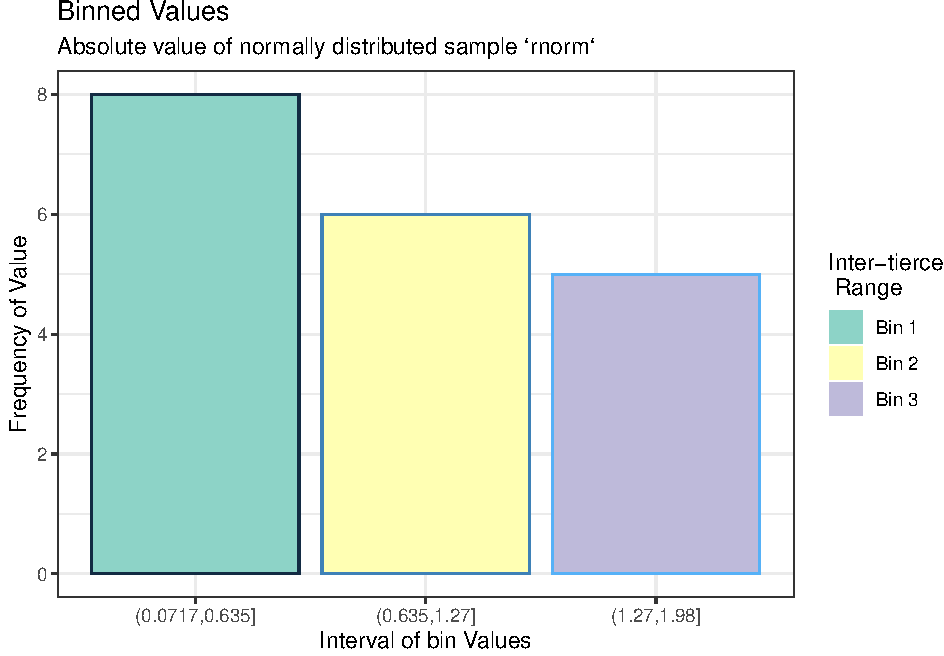
\includegraphics{./figure/unnamed-chunk-7-3.pdf}

remember that this values are absolute values and the skew left
distribution is expected.

\hypertarget{random-sample}{%
\subsubsection{Random Sample}\label{random-sample}}

This is very different from a random sample which could be done like
this:

\begin{Shaded}
\begin{Highlighting}[]
\NormalTok{bin_index <-}\StringTok{ }\KeywordTok{sample}\NormalTok{(}\DecValTok{1}\OperatorTok{:}\DecValTok{3}\NormalTok{, }\DataTypeTok{size =} \KeywordTok{length}\NormalTok{(std_normal), }\DataTypeTok{replace =} \OtherTok{TRUE}\NormalTok{)}

\NormalTok{std_normal_df <-}\StringTok{ }\KeywordTok{as_tibble}\NormalTok{(}\KeywordTok{cbind}\NormalTok{(std_normal, bin_index))}
\CommentTok{# std_normal %>% dplyr::rename("value" = std_normal, "bin" = bin_index)}
\KeywordTok{names}\NormalTok{(std_normal_df) <-}\StringTok{ }\KeywordTok{c}\NormalTok{(}\StringTok{"Value"}\NormalTok{, }\StringTok{"Bin"}\NormalTok{)}
\NormalTok{std_normal_df}\OperatorTok{$}\NormalTok{Bin <-}\StringTok{ }\KeywordTok{factor}\NormalTok{(std_normal_df}\OperatorTok{$}\NormalTok{Bin, }\DataTypeTok{levels =} \DecValTok{1}\OperatorTok{:}\DecValTok{3}\NormalTok{, }\DataTypeTok{ordered =} \OtherTok{FALSE}\NormalTok{)}
\NormalTok{std_normal_df}
\end{Highlighting}
\end{Shaded}

\begin{verbatim}
## # A tibble: 20 x 2
##     Value Bin  
##     <dbl> <fct>
##  1 0.889  2    
##  2 0.382  3    
##  3 0.166  1    
##  4 1.52   2    
##  5 1.38   3    
##  6 1.10   2    
##  7 0.204  1    
##  8 1.77   1    
##  9 0.784  3    
## 10 0.957  3    
## 11 0.312  3    
## 12 1.47   3    
## 13 0.0717 3    
## 14 0.180  3    
## 15 0.113  1    
## 16 0.898  1    
## 17 0.247  3    
## 18 1.03   2    
## 19 1.98   2    
## 20 0.127  3
\end{verbatim}

\begin{Shaded}
\begin{Highlighting}[]
\KeywordTok{summary}\NormalTok{(std_normal_df}\OperatorTok{$}\NormalTok{Bin)}
\end{Highlighting}
\end{Shaded}

\begin{verbatim}
##  1  2  3 
##  5  5 10
\end{verbatim}

\hypertarget{create-a-matrix-of-values}{%
\subsubsection{(4) Create a matrix of
Values}\label{create-a-matrix-of-values}}

this vector can be filled into a matrix, it will fill column wise by
default:

\begin{Shaded}
\begin{Highlighting}[]
\NormalTok{std_normal_mat <-}\StringTok{ }\KeywordTok{matrix}\NormalTok{(}\DataTypeTok{data =}\NormalTok{ std_normal, }\DataTypeTok{nrow =} \DecValTok{3}\NormalTok{, }\DataTypeTok{ncol =} \DecValTok{6}\NormalTok{)}
\end{Highlighting}
\end{Shaded}

\begin{verbatim}
## Warning in base::matrix(...): data length [20] is not a sub-multiple or multiple
## of the number of rows [3]
\end{verbatim}

\begin{Shaded}
\begin{Highlighting}[]
\NormalTok{std_normal_mat}
\end{Highlighting}
\end{Shaded}

\begin{verbatim}
##           [,1]     [,2]      [,3]      [,4]       [,5]      [,6]
## [1,] 0.8890603 1.520310 0.2035836 0.9573273 0.07174706 0.8977332
## [2,] 0.3824008 1.382377 1.7704905 0.3120387 0.18018983 0.2474811
## [3,] 0.1658778 1.103550 0.7843132 1.4741996 0.11261591 1.0260385
\end{verbatim}

In order to fill the matrix row wise it is necessary to specify the
\texttt{byrow} argument:

\begin{Shaded}
\begin{Highlighting}[]
\NormalTok{std_normal_mat <-}\StringTok{ }\KeywordTok{matrix}\NormalTok{(}\DecValTok{1}\OperatorTok{:}\DecValTok{20}\NormalTok{, }\DataTypeTok{nrow =} \DecValTok{3}\NormalTok{, }\DataTypeTok{ncol =} \DecValTok{6}\NormalTok{, }\DataTypeTok{byrow =} \OtherTok{TRUE}\NormalTok{)}
\end{Highlighting}
\end{Shaded}

\begin{verbatim}
## Warning in base::matrix(...): data length [20] is not a sub-multiple or multiple
## of the number of rows [3]
\end{verbatim}

\begin{Shaded}
\begin{Highlighting}[]
\NormalTok{std_normal_mat}
\end{Highlighting}
\end{Shaded}

\begin{verbatim}
##      [,1] [,2] [,3] [,4] [,5] [,6]
## [1,]    1    2    3    4    5    6
## [2,]    7    8    9   10   11   12
## [3,]   13   14   15   16   17   18
\end{verbatim}

\begin{Shaded}
\begin{Highlighting}[]
\NormalTok{std_normal_mat <-}\StringTok{ }\KeywordTok{matrix}\NormalTok{(}\DataTypeTok{data =}\NormalTok{ std_normal, }\DataTypeTok{nrow =} \DecValTok{6}\NormalTok{, }\DataTypeTok{ncol =} \DecValTok{3}\NormalTok{) }\OperatorTok\StringTok{ }\NormalTok{t}
\end{Highlighting}
\end{Shaded}

\begin{verbatim}
## Warning in base::matrix(...): data length [20] is not a sub-multiple or multiple
## of the number of rows [6]
\end{verbatim}

\begin{Shaded}
\begin{Highlighting}[]
\NormalTok{std_normal_mat}
\end{Highlighting}
\end{Shaded}

\begin{verbatim}
##            [,1]      [,2]      [,3]      [,4]      [,5]     [,6]
## [1,] 0.88906032 0.3824008 0.1658778 1.5203096 1.3823774 1.103550
## [2,] 0.20358362 1.7704905 0.7843132 0.9573273 0.3120387 1.474200
## [3,] 0.07174706 0.1801898 0.1126159 0.8977332 0.2474811 1.026038
\end{verbatim}

alternatively it would also be possible to transpose the data:

\begin{Shaded}
\begin{Highlighting}[]
\NormalTok{std_normal_mat <-}\StringTok{ }\KeywordTok{matrix}\NormalTok{(}\DataTypeTok{data =} \DecValTok{1}\OperatorTok{:}\DecValTok{20}\NormalTok{ , }\DataTypeTok{nrow =} \DecValTok{6}\NormalTok{, }\DataTypeTok{ncol =} \DecValTok{3}\NormalTok{) }\OperatorTok\StringTok{ }\NormalTok{t}
\end{Highlighting}
\end{Shaded}

\begin{verbatim}
## Warning in base::matrix(...): data length [20] is not a sub-multiple or multiple
## of the number of rows [6]
\end{verbatim}

\begin{Shaded}
\begin{Highlighting}[]
\NormalTok{std_normal_mat}
\end{Highlighting}
\end{Shaded}

\begin{verbatim}
##      [,1] [,2] [,3] [,4] [,5] [,6]
## [1,]    1    2    3    4    5    6
## [2,]    7    8    9   10   11   12
## [3,]   13   14   15   16   17   18
\end{verbatim}

\begin{Shaded}
\begin{Highlighting}[]
\NormalTok{std_normal_mat <-}\StringTok{ }\KeywordTok{matrix}\NormalTok{(}\DataTypeTok{data =}\NormalTok{ std_normal, }\DataTypeTok{nrow =} \DecValTok{6}\NormalTok{, }\DataTypeTok{ncol =} \DecValTok{3}\NormalTok{) }\OperatorTok\StringTok{ }\NormalTok{t}
\end{Highlighting}
\end{Shaded}

\begin{verbatim}
## Warning in base::matrix(...): data length [20] is not a sub-multiple or multiple
## of the number of rows [6]
\end{verbatim}

\begin{Shaded}
\begin{Highlighting}[]
\NormalTok{std_normal_mat}
\end{Highlighting}
\end{Shaded}

\begin{verbatim}
##            [,1]      [,2]      [,3]      [,4]      [,5]     [,6]
## [1,] 0.88906032 0.3824008 0.1658778 1.5203096 1.3823774 1.103550
## [2,] 0.20358362 1.7704905 0.7843132 0.9573273 0.3120387 1.474200
## [3,] 0.07174706 0.1801898 0.1126159 0.8977332 0.2474811 1.026038
\end{verbatim}

\hypertarget{linear-regression}{%
\subsection{(5) Linear Regression}\label{linear-regression}}

\hypertarget{base-packages}{%
\subsubsection{Base Packages}\label{base-packages}}

Using Base Packages Speed and Distance may be plotted thusly:

\begin{Shaded}
\begin{Highlighting}[]
\NormalTok{carsForm <-}\StringTok{ }\NormalTok{dist }\OperatorTok{~}\StringTok{ }\NormalTok{speed}
\NormalTok{cars_model <-}\StringTok{ }\KeywordTok{lm}\NormalTok{(}\DataTypeTok{formula =}\NormalTok{ carsForm, }\DataTypeTok{data =}\NormalTok{ cars)}

\KeywordTok{plot}\NormalTok{(dist }\OperatorTok{~}\StringTok{ }\NormalTok{speed, }\DataTypeTok{data =}\NormalTok{ cars,}
     \DataTypeTok{main =} \StringTok{"Stopping Distance and Speed"}\NormalTok{,}
     \DataTypeTok{ylab =} \StringTok{"Stopping Distance"}\NormalTok{,}
     \DataTypeTok{xlab =} \StringTok{"Vehicle Speed"}\NormalTok{,}
     \DataTypeTok{bg =} \StringTok{"red"}\NormalTok{,}
     \DataTypeTok{pch =} \StringTok{"&"}\NormalTok{, }\DataTypeTok{cex =} \DecValTok{2}\NormalTok{,}
     \DataTypeTok{col =} \StringTok{"purple"}\NormalTok{)}

\KeywordTok{abline}\NormalTok{(cars_model, }\DataTypeTok{lty =} \DecValTok{3}\NormalTok{, }\DataTypeTok{lwd =} \DecValTok{7}\NormalTok{, }\DataTypeTok{col =} \StringTok{"red"}\NormalTok{)}
\end{Highlighting}
\end{Shaded}

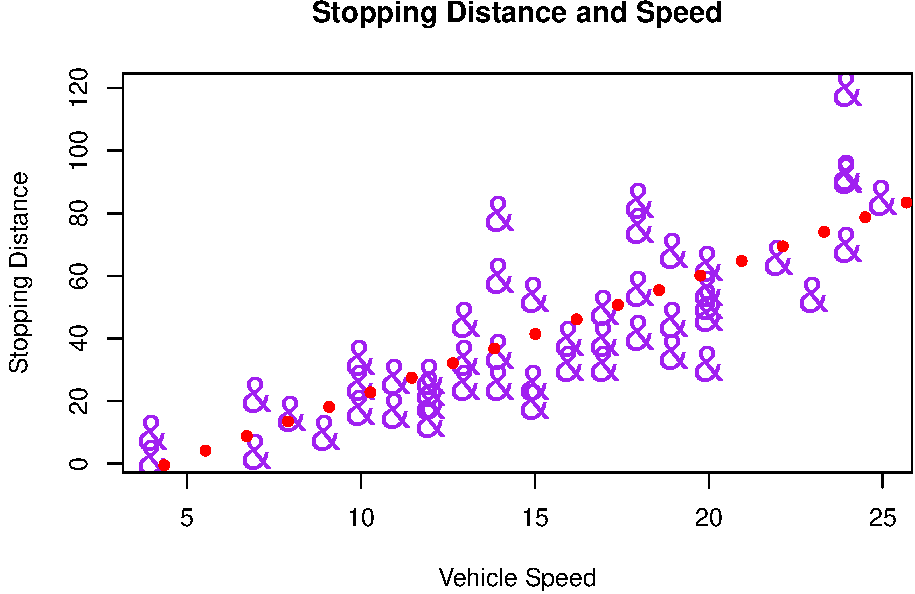
\includegraphics{./figure/unnamed-chunk-12-1.pdf}

Values can be forecast using the \texttt{predict()} function:

\begin{Shaded}
\begin{Highlighting}[]
\KeywordTok{names}\NormalTok{(cars)}
\end{Highlighting}
\end{Shaded}

\begin{verbatim}
## [1] "speed" "dist"
\end{verbatim}

\begin{Shaded}
\begin{Highlighting}[]
\KeywordTok{attach}\NormalTok{(cars)}
\KeywordTok{predict}\NormalTok{(cars_model, }\DataTypeTok{newdata =} \KeywordTok{data.frame}\NormalTok{(}\DataTypeTok{speed =} \DecValTok{40}\NormalTok{))}
\end{Highlighting}
\end{Shaded}

\begin{verbatim}
##        1 
## 139.7173
\end{verbatim}

\begin{Shaded}
\begin{Highlighting}[]
\KeywordTok{detach}\NormalTok{(cars)}
\end{Highlighting}
\end{Shaded}

This can then be added onto the plot using \texttt{points()}:

\begin{Shaded}
\begin{Highlighting}[]
\CommentTok{# Increase the Plot Limit}

\KeywordTok{plot}\NormalTok{(dist }\OperatorTok{~}\StringTok{ }\NormalTok{speed, }\DataTypeTok{data =}\NormalTok{ cars,}
     \DataTypeTok{main =} \StringTok{"Stopping Distance and Speed"}\NormalTok{,}
     \DataTypeTok{ylab =} \StringTok{"Stopping Distance"}\NormalTok{,}
     \DataTypeTok{xlab =} \StringTok{"Vehicle Speed"}\NormalTok{,}
     \DataTypeTok{bg =} \StringTok{"red"}\NormalTok{,}
     \DataTypeTok{pch =} \StringTok{"&"}\NormalTok{, }\DataTypeTok{cex =} \DecValTok{2}\NormalTok{,}
     \DataTypeTok{col =} \StringTok{"purple"}\NormalTok{, }
     \DataTypeTok{xlim =} \KeywordTok{c}\NormalTok{(}\DecValTok{0}\NormalTok{, }\DecValTok{40}\NormalTok{), }
     \DataTypeTok{ylim =} \KeywordTok{c}\NormalTok{(}\DecValTok{0}\NormalTok{, }\DecValTok{140}\NormalTok{))}

\KeywordTok{abline}\NormalTok{(cars_model, }\DataTypeTok{lty =} \DecValTok{3}\NormalTok{, }\DataTypeTok{lwd =} \DecValTok{7}\NormalTok{, }\DataTypeTok{col =} \StringTok{"blue"}\NormalTok{)}
\KeywordTok{points}\NormalTok{(}\DecValTok{40}\NormalTok{, }\DecValTok{140}\NormalTok{, }\DataTypeTok{pch =} \DecValTok{9}\NormalTok{, }\DataTypeTok{cex =} \DecValTok{3}\NormalTok{, }\DataTypeTok{col =} \StringTok{"red"}\NormalTok{)}
\end{Highlighting}
\end{Shaded}

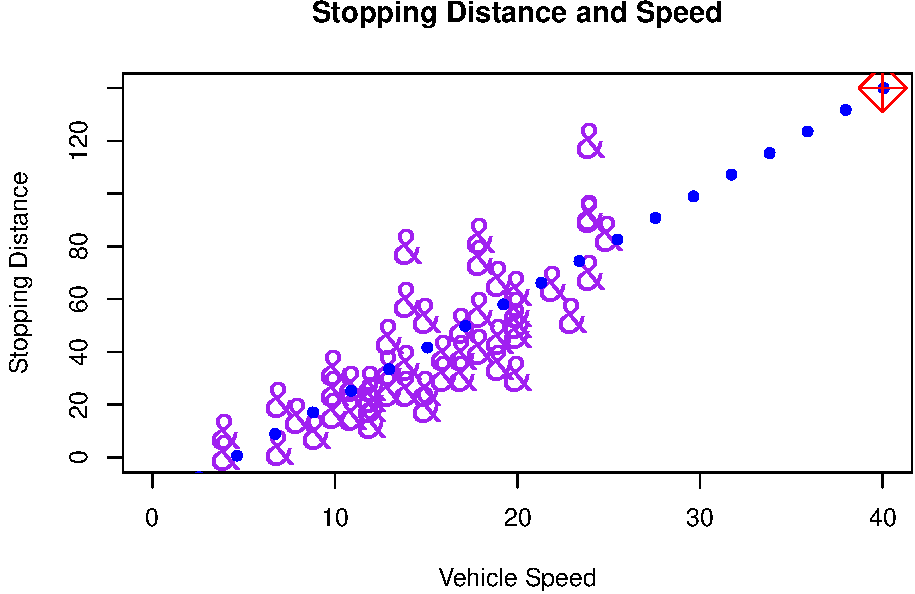
\includegraphics{./figure/unnamed-chunk-14-1.pdf}

\hypertarget{ggplot2}{%
\subsubsection{GGPlot2}\label{ggplot2}}

This is a little simpler in ggplot2.

\hypertarget{build-the-model}{%
\paragraph{Build the Model}\label{build-the-model}}

\begin{Shaded}
\begin{Highlighting}[]
\NormalTok{cars_model <-}\StringTok{ }\KeywordTok{lm}\NormalTok{(dist }\OperatorTok{~}\StringTok{ }\NormalTok{speed, }\DataTypeTok{data =}\NormalTok{ cars)}
\KeywordTok{summary}\NormalTok{(cars_model)}
\end{Highlighting}
\end{Shaded}

\begin{verbatim}
## 
## Call:
## lm(formula = dist ~ speed, data = cars)
## 
## Residuals:
##     Min      1Q  Median      3Q     Max 
## -29.069  -9.525  -2.272   9.215  43.201 
## 
## Coefficients:
##             Estimate Std. Error t value Pr(>|t|)    
## (Intercept) -17.5791     6.7584  -2.601   0.0123 *  
## speed         3.9324     0.4155   9.464 1.49e-12 ***
## ---
## Signif. codes:  0 '***' 0.001 '**' 0.01 '*' 0.05 '.' 0.1 ' ' 1
## 
## Residual standard error: 15.38 on 48 degrees of freedom
## Multiple R-squared:  0.6511, Adjusted R-squared:  0.6438 
## F-statistic: 89.57 on 1 and 48 DF,  p-value: 1.49e-12
\end{verbatim}

\[
\texttt{dist} = 0.017 \times \texttt{speed } + 8.28
\] \#\#\#\# Create some Predictions

\begin{Shaded}
\begin{Highlighting}[]
\KeywordTok{max}\NormalTok{(cars}\OperatorTok{$}\NormalTok{speed)}
\end{Highlighting}
\end{Shaded}

\begin{verbatim}
## [1] 25
\end{verbatim}

\begin{Shaded}
\begin{Highlighting}[]
\NormalTok{newdata <-}\StringTok{ }\KeywordTok{data.frame}\NormalTok{(}\DataTypeTok{speed =} \KeywordTok{c}\NormalTok{(}\DecValTok{30}\NormalTok{, }\DecValTok{33}\NormalTok{, }\DecValTok{37}\NormalTok{))}
\NormalTok{newdata}\OperatorTok{$}\NormalTok{dist <-}\StringTok{ }\KeywordTok{predict}\NormalTok{(}\DataTypeTok{object =}\NormalTok{ cars_model, newdata)}
\NormalTok{newdata}\OperatorTok{$}\NormalTok{datatype <-}\StringTok{ }\KeywordTok{c}\NormalTok{(}\StringTok{"pred"}\NormalTok{)}

\NormalTok{cars}\OperatorTok{$}\NormalTok{datatype <-}\StringTok{ }\KeywordTok{c}\NormalTok{(}\StringTok{"obs"}\NormalTok{)}

\NormalTok{cars <-}\StringTok{ }\KeywordTok{rbind}\NormalTok{(cars, newdata)}
\NormalTok{cars}\OperatorTok{$}\NormalTok{datatype <-}\StringTok{ }\KeywordTok{factor}\NormalTok{(cars}\OperatorTok{$}\NormalTok{datatype)}
\KeywordTok{head}\NormalTok{(cars)}
\end{Highlighting}
\end{Shaded}

\begin{verbatim}
##   speed dist datatype
## 1     4    2      obs
## 2     4   10      obs
## 3     7    4      obs
## 4     7   22      obs
## 5     8   16      obs
## 6     9   10      obs
\end{verbatim}

\hypertarget{plot-the-data-type}{%
\paragraph{Plot the Data Type}\label{plot-the-data-type}}

\begin{Shaded}
\begin{Highlighting}[]
\KeywordTok{ggplot}\NormalTok{(}\DataTypeTok{data =}\NormalTok{ cars, }\KeywordTok{aes}\NormalTok{(}\DataTypeTok{x =}\NormalTok{ speed, }\DataTypeTok{y =}\NormalTok{ dist, }\DataTypeTok{col =}\NormalTok{ datatype)) }\OperatorTok{+}
\StringTok{  }\KeywordTok{geom_point}\NormalTok{(}\KeywordTok{aes}\NormalTok{(}\DataTypeTok{size =} \DecValTok{3}\NormalTok{)) }\OperatorTok{+}
\StringTok{  }\KeywordTok{theme_classic}\NormalTok{() }\OperatorTok{+}
\StringTok{  }\KeywordTok{guides}\NormalTok{(}\DataTypeTok{size =} \OtherTok{FALSE}\NormalTok{) }\OperatorTok{+}
\StringTok{  }\KeywordTok{stat_smooth}\NormalTok{(}\DataTypeTok{method =}\NormalTok{ lm, }\KeywordTok{aes}\NormalTok{(}\DataTypeTok{group =} \DecValTok{1}\NormalTok{), }\DataTypeTok{se =} \OtherTok{FALSE}\NormalTok{, }\DataTypeTok{lty =} \DecValTok{2}\NormalTok{) }\OperatorTok{+}
\StringTok{  }\KeywordTok{labs}\NormalTok{(}\DataTypeTok{x =} \StringTok{"Velocity of Vehicle"}\NormalTok{, }\DataTypeTok{y =} \StringTok{"Breaking Distance"}\NormalTok{, }\DataTypeTok{title =} \StringTok{"Vehicle Breaking"}\NormalTok{) }\OperatorTok{+}
\StringTok{  }\KeywordTok{guides}\NormalTok{(}\DataTypeTok{col =} \KeywordTok{guide_legend}\NormalTok{(}\StringTok{"Data Type"}\NormalTok{)) }\OperatorTok{+}\StringTok{ }
\StringTok{  }\KeywordTok{scale_color_discrete}\NormalTok{(}\DataTypeTok{labels =} \KeywordTok{c}\NormalTok{(}\StringTok{"Observation"}\NormalTok{, }\StringTok{"Prediction"}\NormalTok{)) }\OperatorTok{+}
\StringTok{  }\KeywordTok{scale_color_manual}\NormalTok{(}\DataTypeTok{labels =} \KeywordTok{c}\NormalTok{(}\StringTok{"Observation"}\NormalTok{, }\StringTok{"Prediction"}\NormalTok{),}
                     \DataTypeTok{values =} \KeywordTok{c}\NormalTok{(}\StringTok{"indianred"}\NormalTok{, }\StringTok{"royalblue"}\NormalTok{))}
\end{Highlighting}
\end{Shaded}

\begin{verbatim}
## Scale for 'colour' is already present. Adding another scale for 'colour',
## which will replace the existing scale.
\end{verbatim}

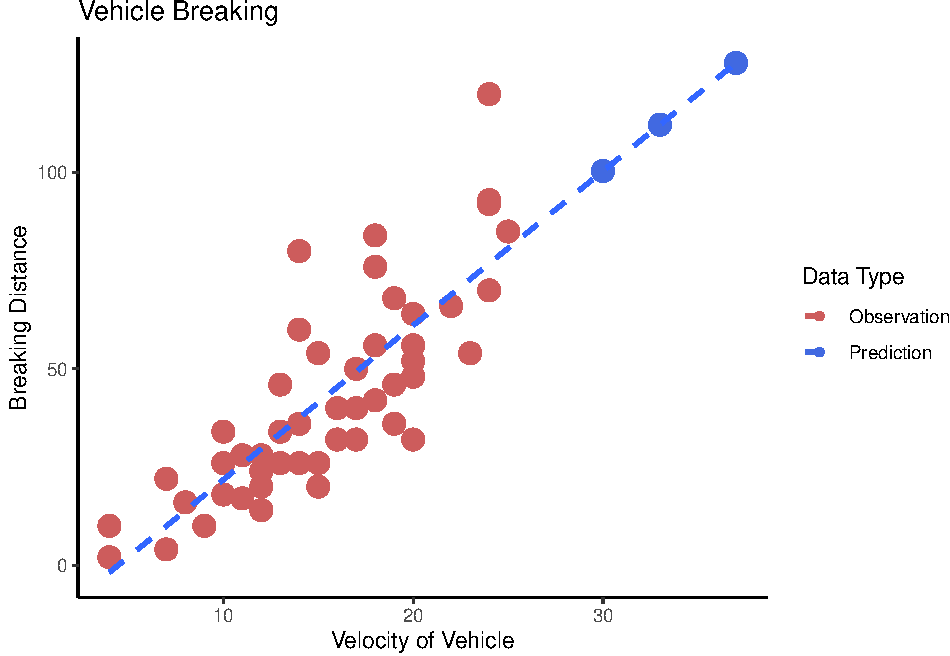
\includegraphics{./figure/unnamed-chunk-17-1.pdf}

\hypertarget{refine-the-model}{%
\subparagraph{Refine the Model}\label{refine-the-model}}

A car break transforms the kinetic energy of the car into thermal energy
in the break rotor:

\[\begin{aligned}
E_\textsf{Brk} &= E_\textsf{Car} \\
F\cdot  s  &= \frac{1}{2}\cdot  m\cdot  v^2 \\
 \implies  s &=  \frac{m\cdot  F}{s} \cdot  v^2 \\
 s & \propto v^2
\end{aligned}\]

Another way to look at this model, as opposed to a conservation of
energy argument is to consider the distance travelled while breaking as
a function of the force applied by the break.

Assume that the breaking force of the car is constant, if the breaking
system of any given car is adjusted to be stronger for heavier cars such
that the deceleration is constant for any car regardless of mass the
following simplification can be used where \(a\) represents the
deceleration caused by breaking:

\[\begin{aligned}
F &=  m\cdot  a \\
\implies  F &\propto a
\end{aligned}\]

and hence the distance travelled while breaking will be

\[\begin{aligned}
v &=  a \cdot   t \\
\int v \mathrm{d}t &=  \int a\cdot t \mathrm{d}t  \\
s&= \frac{1}{2}a\cdot  t^2 \\
2s &= a\cdot  \left( \frac{v}{a} \right)^2\\
2as &= v^2
\end{aligned}\]

Under the assumption that deceleratoin is constant:

\[\begin{aligned}
s \propto v^2
\end{aligned}\]

using \texttt{stat\_smooth}

This can be added by using the stats layer in ggplot2, simply add
\texttt{formula\ =\ y\ \textasciitilde{}\ I(x\^{}2)} to the
\texttt{stat\_smooth} lm layer:

\begin{quote}
remember that it is a linear model in the sense that a linear model is
simply fit to a new variable that just so happens to be the square of
the original data, the method used is still Ordinary Least Squares
Regression, refer to
\href{/home/ryan/Dropbox/Studies/Old/Studies(ONote)/Statistics/Data\%20Science/PredMod/Proofs/Number\%20Theory/Simple\%20Linear\%20Regression.pdf}{This
Document} for a proof.
\end{quote}

\begin{Shaded}
\begin{Highlighting}[]
\CommentTok{# cars <- cars %>% dplyr::filter("obs" %in% datatype)}
\CommentTok{# cars <- cars[cars$datatype == "obs",] }
\KeywordTok{ggplot}\NormalTok{(}\DataTypeTok{data =}\NormalTok{ cars, }\KeywordTok{aes}\NormalTok{(}\DataTypeTok{x =}\NormalTok{ speed, }\DataTypeTok{y =}\NormalTok{ dist, }\DataTypeTok{col =}\NormalTok{ datatype)) }\OperatorTok{+}
\StringTok{  }\KeywordTok{geom_point}\NormalTok{(}\KeywordTok{aes}\NormalTok{(}\DataTypeTok{size =} \DecValTok{3}\NormalTok{)) }\OperatorTok{+}
\StringTok{  }\KeywordTok{theme_classic}\NormalTok{() }\OperatorTok{+}
\StringTok{  }\KeywordTok{guides}\NormalTok{(}\DataTypeTok{size =} \OtherTok{FALSE}\NormalTok{) }\OperatorTok{+}
\StringTok{  }\KeywordTok{stat_smooth}\NormalTok{(}\DataTypeTok{method =}\NormalTok{ lm, }\KeywordTok{aes}\NormalTok{(}\DataTypeTok{group =} \DecValTok{1}\NormalTok{), }\DataTypeTok{formula =}\NormalTok{ y }\OperatorTok{~}\StringTok{ }\KeywordTok{I}\NormalTok{(x}\OperatorTok{^}\DecValTok{2}\NormalTok{), }\DataTypeTok{se =} \OtherTok{FALSE}\NormalTok{, }\DataTypeTok{lty =} \DecValTok{2}\NormalTok{, }\DataTypeTok{col =} \StringTok{"purple"}\NormalTok{) }\OperatorTok{+}
\StringTok{  }\KeywordTok{labs}\NormalTok{(}\DataTypeTok{x =} \StringTok{"Velocity of Vehicle"}\NormalTok{, }\DataTypeTok{y =} \StringTok{"Breaking Distance"}\NormalTok{, }\DataTypeTok{title =} \StringTok{"Vehicle Breaking"}\NormalTok{) }\OperatorTok{+}
\StringTok{  }\KeywordTok{guides}\NormalTok{(}\DataTypeTok{col =} \KeywordTok{guide_legend}\NormalTok{(}\StringTok{"Data Type"}\NormalTok{)) }\OperatorTok{+}\StringTok{ }
\StringTok{  }\KeywordTok{scale_color_discrete}\NormalTok{(}\DataTypeTok{labels =} \KeywordTok{c}\NormalTok{(}\StringTok{"Observation"}\NormalTok{, }\StringTok{"Prediction"}\NormalTok{)) }\OperatorTok{+}
\StringTok{  }\KeywordTok{scale_color_manual}\NormalTok{(}\DataTypeTok{labels =} \KeywordTok{c}\NormalTok{(}\StringTok{"Observation"}\NormalTok{, }\StringTok{"Linear Prediction"}\NormalTok{),}
                     \DataTypeTok{values =} \KeywordTok{c}\NormalTok{(}\StringTok{"indianred"}\NormalTok{, }\StringTok{"royalblue"}\NormalTok{))}
\end{Highlighting}
\end{Shaded}

\begin{verbatim}
## Scale for 'colour' is already present. Adding another scale for 'colour',
## which will replace the existing scale.
\end{verbatim}

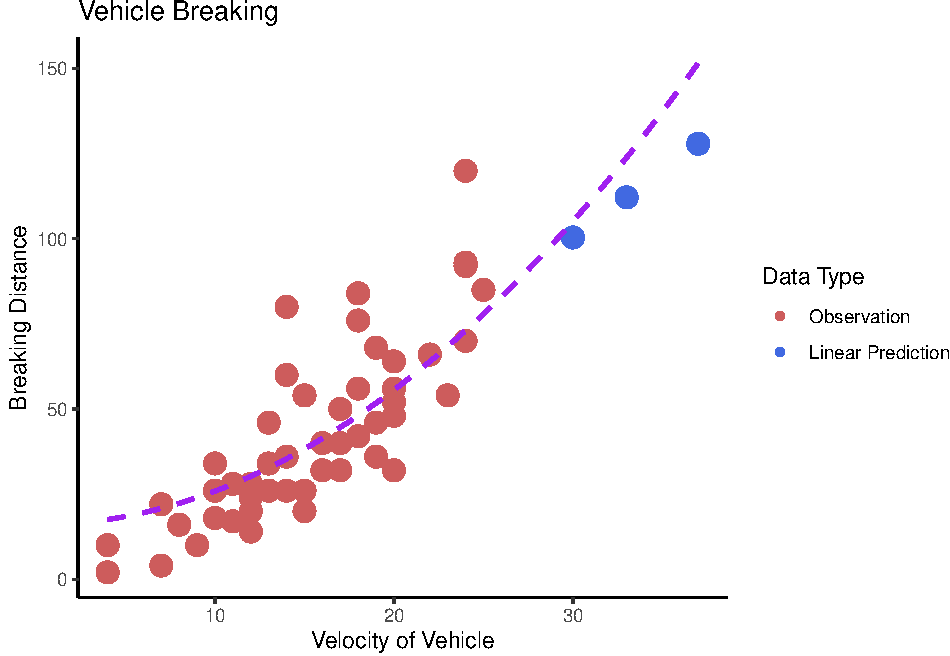
\includegraphics{./figure/unnamed-chunk-18-1.pdf}

Build the Model

If more precise control was necessary for the model that was built, a
seperate data set can simply be plotted over the top of the data in a
seperate layer like so:

\begin{Shaded}
\begin{Highlighting}[]
\NormalTok{cars_model <-}\StringTok{ }\KeywordTok{lm}\NormalTok{(dist }\OperatorTok{~}\StringTok{ }\KeywordTok{poly}\NormalTok{(speed, }\DataTypeTok{degree =} \DecValTok{2}\NormalTok{, }\DataTypeTok{raw =} \OtherTok{TRUE}\NormalTok{), }\DataTypeTok{data =}\NormalTok{ cars)}
\KeywordTok{summary}\NormalTok{(cars_model)}
\end{Highlighting}
\end{Shaded}

\begin{verbatim}
## 
## Call:
## lm(formula = dist ~ poly(speed, degree = 2, raw = TRUE), data = cars)
## 
## Residuals:
##     Min      1Q  Median      3Q     Max 
## -28.033  -8.920  -2.095   4.484  43.668 
## 
## Coefficients:
##                                       Estimate Std. Error t value Pr(>|t|)  
## (Intercept)                          -10.95719   10.75299  -1.019   0.3131  
## poly(speed, degree = 2, raw = TRUE)1   3.11171    1.18526   2.625   0.0115 *
## poly(speed, degree = 2, raw = TRUE)2   0.02189    0.03049   0.718   0.4762  
## ---
## Signif. codes:  0 '***' 0.001 '**' 0.01 '*' 0.05 '.' 0.1 ' ' 1
## 
## Residual standard error: 14.99 on 50 degrees of freedom
## Multiple R-squared:  0.7609, Adjusted R-squared:  0.7513 
## F-statistic: 79.55 on 2 and 50 DF,  p-value: 2.921e-16
\end{verbatim}

\[
\texttt{dist} = 0.099 \times \texttt{speed}^2 + 0.91 \times \texttt{speed} + 2.4
\]

This can be added to ggplot2 by just using geom\_line over the modelled
like so:

\begin{Shaded}
\begin{Highlighting}[]
\NormalTok{cars}\OperatorTok{$}\NormalTok{quad <-}\StringTok{ }\KeywordTok{predict}\NormalTok{(cars_model, }\DataTypeTok{newdata =} \KeywordTok{data.frame}\NormalTok{(}\StringTok{"speed"}\NormalTok{=cars[,}\KeywordTok{names}\NormalTok{(cars) }\OperatorTok{==}\StringTok{ "speed"}\NormalTok{]))}

\NormalTok{quad_model_df <-}\StringTok{ }\KeywordTok{tibble}\NormalTok{(}\StringTok{"speed"}\NormalTok{ =}\StringTok{ }\DecValTok{1}\OperatorTok{:}\DecValTok{40}\NormalTok{)}
\NormalTok{quad_model_df}\OperatorTok{$}\NormalTok{distq <-}\StringTok{ }\KeywordTok{predict}\NormalTok{(}\DataTypeTok{object =}\NormalTok{ cars_model, }\DataTypeTok{newdata =}\NormalTok{ quad_model_df)}

\KeywordTok{ggplot}\NormalTok{(}\DataTypeTok{data =}\NormalTok{ cars, }\KeywordTok{aes}\NormalTok{(}\DataTypeTok{x =}\NormalTok{ speed, }\DataTypeTok{y =}\NormalTok{ dist)) }\OperatorTok{+}
\StringTok{  }\KeywordTok{geom_point}\NormalTok{(}\KeywordTok{aes}\NormalTok{(}\DataTypeTok{size =} \DecValTok{3}\NormalTok{, }\DataTypeTok{col =}\NormalTok{ datatype)) }\OperatorTok{+}
\StringTok{  }\KeywordTok{theme_classic}\NormalTok{() }\OperatorTok{+}
\StringTok{  }\KeywordTok{guides}\NormalTok{(}\DataTypeTok{size =} \OtherTok{FALSE}\NormalTok{) }\OperatorTok{+}
\StringTok{  }\KeywordTok{stat_smooth}\NormalTok{(}\DataTypeTok{method =}\NormalTok{ lm, }\KeywordTok{aes}\NormalTok{(}\DataTypeTok{group =} \DecValTok{1}\NormalTok{), }\DataTypeTok{se =} \OtherTok{FALSE}\NormalTok{, }\DataTypeTok{lty =} \DecValTok{2}\NormalTok{) }\OperatorTok{+}
\StringTok{  }\KeywordTok{labs}\NormalTok{(}\DataTypeTok{x =} \StringTok{"Velocity of Vehicle"}\NormalTok{, }\DataTypeTok{y =} \StringTok{"Breaking Distance"}\NormalTok{, }\DataTypeTok{title =} \StringTok{"Vehicle Breaking"}\NormalTok{) }\OperatorTok{+}
\StringTok{  }\KeywordTok{guides}\NormalTok{(}\DataTypeTok{col =} \KeywordTok{guide_legend}\NormalTok{(}\StringTok{"Data Type"}\NormalTok{)) }\OperatorTok{+}\StringTok{ }
\StringTok{  }\KeywordTok{scale_color_discrete}\NormalTok{(}\DataTypeTok{labels =} \KeywordTok{c}\NormalTok{(}\StringTok{"Observation"}\NormalTok{, }\StringTok{"Prediction"}\NormalTok{)) }\OperatorTok{+}
\StringTok{  }\KeywordTok{scale_color_manual}\NormalTok{(}\DataTypeTok{labels =} \KeywordTok{c}\NormalTok{(}\StringTok{"Observation"}\NormalTok{, }\StringTok{"Prediction"}\NormalTok{),}
                     \DataTypeTok{values =} \KeywordTok{c}\NormalTok{(}\StringTok{"indianred"}\NormalTok{, }\StringTok{"royalblue"}\NormalTok{)) }\OperatorTok{+}
\StringTok{  }\KeywordTok{geom_line}\NormalTok{(}\DataTypeTok{data =}\NormalTok{ quad_model_df, }\KeywordTok{aes}\NormalTok{(}\DataTypeTok{x =}\NormalTok{ speed, }\DataTypeTok{y =}\NormalTok{ distq), }\DataTypeTok{col =} \StringTok{"purple"}\NormalTok{, }\DataTypeTok{lty =}\DecValTok{2}\NormalTok{)}
\end{Highlighting}
\end{Shaded}

\begin{verbatim}
## Scale for 'colour' is already present. Adding another scale for 'colour',
## which will replace the existing scale.
\end{verbatim}

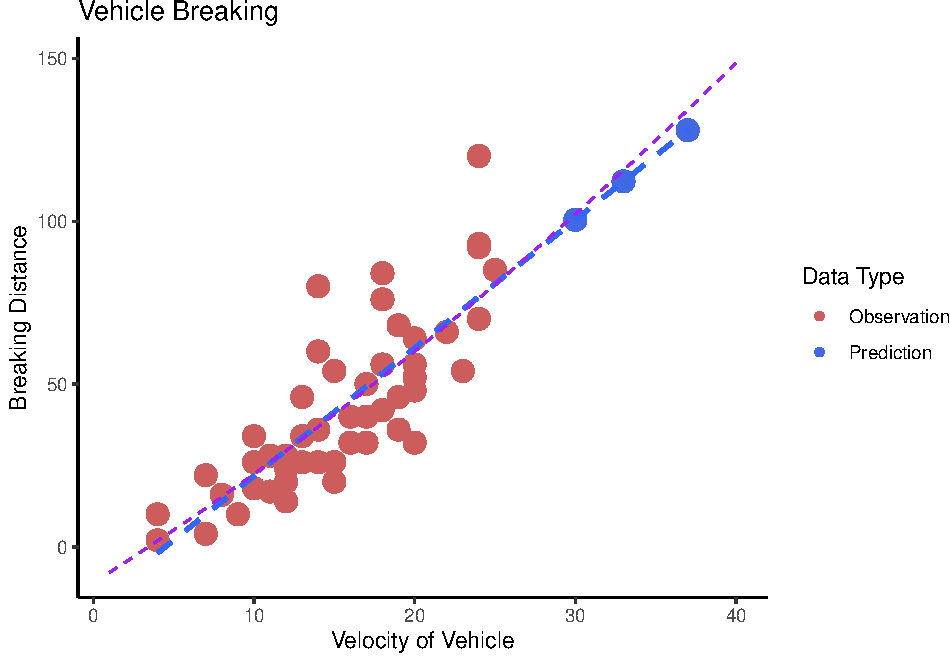
\includegraphics{./figure/unnamed-chunk-20-1.pdf}


\end{document}
